%% LyX 2.2.3 created this file.  For more info, see http://www.lyx.org/.
%% Do not edit unless you really know what you are doing.
\documentclass[czech]{beamer}
\usepackage[T1]{fontenc}
\usepackage[utf8]{inputenc}
\setcounter{secnumdepth}{3}
\setcounter{tocdepth}{3}
\usepackage{graphicx}

\makeatletter

%%%%%%%%%%%%%%%%%%%%%%%%%%%%%% LyX specific LaTeX commands.
\newcommand{\noun}[1]{\textsc{#1}}

%%%%%%%%%%%%%%%%%%%%%%%%%%%%%% Textclass specific LaTeX commands.
 % this default might be overridden by plain title style
 \newcommand\makebeamertitle{\frame{\maketitle}}%
 % (ERT) argument for the TOC
 \AtBeginDocument{%
   \let\origtableofcontents=\tableofcontents
   \def\tableofcontents{\@ifnextchar[{\origtableofcontents}{\gobbletableofcontents}}
   \def\gobbletableofcontents#1{\origtableofcontents}
 }
 % plain title style, override default
 \renewcommand\makebeamertitle{\frame[plain]{\maketitle}}%

%%%%%%%%%%%%%%%%%%%%%%%%%%%%%% User specified LaTeX commands.
\usepackage{minted}
\usetheme{Antibes}
\usecolortheme{crane}

\makeatother

\usepackage{babel}
\begin{document}

\title{Webový systém pro testování znalostí studentů}

\subtitle{Výzkumný úkol}

\titlegraphic{
\includegraphics{symbol_cvut_konturova_verze_cb}}

\author{Bc. František Navrkal}

\institute{České vysoké učení technické v Praze, Fakulta jaderná a fyzikálně
inženýrská}

\date{2017-09-14}
\makebeamertitle

\section*{Úvod}

\subsection*{Obsah práce}
%
\begin{frame}{O čem je výzkumný úkol?}

%
Cíle práce (ze zadání):
\begin{itemize}
\item prostudovat teorii adaptivního testování znalostí a bayesovských sítí,
\item navrhnout a realizovat webový systém pro realizaci adaptivního testování
(systém má obsahovat i GUI, nástroje pro analýzu výsledků a sběr dat).
\end{itemize}
Cíle práce (de facto):
\begin{itemize}
\item nastínit základní koncepty nutné pro pochopení fungování aplikace,
\item ukázat postup pro návrh adaptivního testu,
\item stručně zdokumentovat aplikaci.
\end{itemize}
\end{frame}
%

\section{Počítačové adaptivní testování}

\subsection{Obecný popis a motivace}
\begin{frame}{Počítačové adaptivní testování}


Přizpůsobování testu na základě informací o studentovi
\begin{itemize}
\item z průběhu testu a
\item z ostatních údajů o studentovi.
\end{itemize}
Motivace:
\begin{itemize}
\item nutno pokrýt všechny úrovně dovedností,
\item odstranění nudy a nepozornosti u zdatných studenty,
\item odstranění zmatku, frustrace, náhodně uhodnutých odpovědí u těch méně
zdatných.
\end{itemize}
\end{frame}

\section{Bayesovské sítě}

\subsection{Obecný popis}
\begin{frame}{Bayesovské sítě}


Pravděpodobnostní datový model popisující kauzální vztahy mezi náhodnými
veličinami.
\begin{itemize}
\item Struktura:
\begin{itemize}
\item orientovaný acyklický graf.
\end{itemize}
\item Podmíněné pravděpodobnosti:
\begin{itemize}
\item funkce pravděpodobnostních rozdělení náhodných veličin
\item nebo speciálně tabulky podmíněných pravděpodobností.
\end{itemize}
\end{itemize}
\end{frame}

\subsection{Příklady}

\begin{frame}{Struktura pro testování znalostí z angličtiny}


\begin{center}
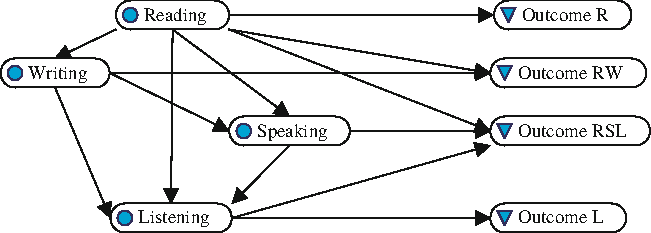
\includegraphics{almond_BN_example}
\par\end{center}

\begin{center}
{\footnotesize{}Zdroj: ALMOND, R.G., MISLEVY, R.J., STEINBERG, L.,
YAN, D., WILLIAMSON, D. Bayesian Networks in Educational Assessment.
Springer, 2015.}
\par\end{center}{\footnotesize \par}

\end{frame}
%
\begin{frame}{Struktura pro testování znalostí z matematiky}


\begin{center}
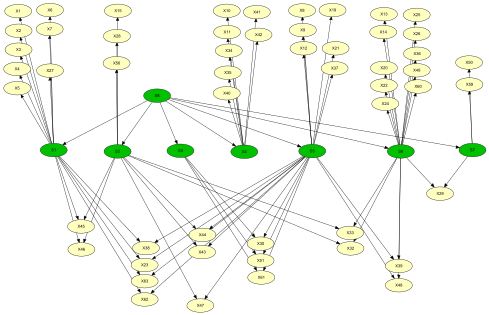
\includegraphics[scale=0.65]{complex_BN_plajner16}
\par\end{center}

\begin{center}
{\scriptsize{}Zdroj: PLAJNER, M., J. VOMLEL. Student Skill Models
in Adaptive Testing. Proceedings of the Eighth International Conference
on Probabilistic Graphical Models, pp. 403–414, 2016.}
\par\end{center}{\scriptsize \par}
\end{frame}

\section{Návrh testu}

\subsection{Obecný postup}
\begin{frame}{Možný postup návrhu adaptivního testu}


\begin{enumerate}
\item Návrh otázek a kandidátních struktur bayesovské sítě,
\item získání dat pomocí statických testů,
\item naučení tabulek podmíněných pravděpodobností,
\item porovnání modelů.
\end{enumerate}
\end{frame}
%
\begin{frame}{Srovnání výkonu modelů}


\begin{center}
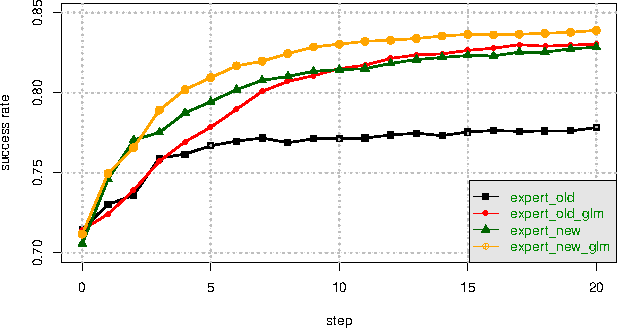
\includegraphics[scale=0.9]{comparison_chart_plajner16}
\par\end{center}

\begin{center}
{\scriptsize{}Zdroj: PLAJNER, M., J. VOMLEL. Student Skill Models
in Adaptive Testing. Proceedings of the Eighth International Conference
on Probabilistic Graphical Models, pp. 403–414, 2016.}
\par\end{center}{\scriptsize \par}
\end{frame}

\section{Vyvíjený systém}

\subsection{Struktura systému}
\begin{frame}{Struktura systému}


\begin{enumerate}
\item Aplikace samotná, napsaná v \textit{Pythonu} – v podstatě moje vlastní
knihovna \noun{CArisTotle} –,
\item SQL databáze, přistupovaná přes \emph{SQLAlchemy}, – nyní pro vývoj
\emph{SQLite} –,
\item knihovna \noun{catest} v \emph{R}, spojená přes \emph{RPy2} se zbytkem
systému a
\item \emph{Jinja} šablony pro tvorbu výstupního HTML kódu.
\end{enumerate}
\end{frame}

\subsection{Datový model}
\begin{frame}{Datový model (1/3)}


\begin{center}
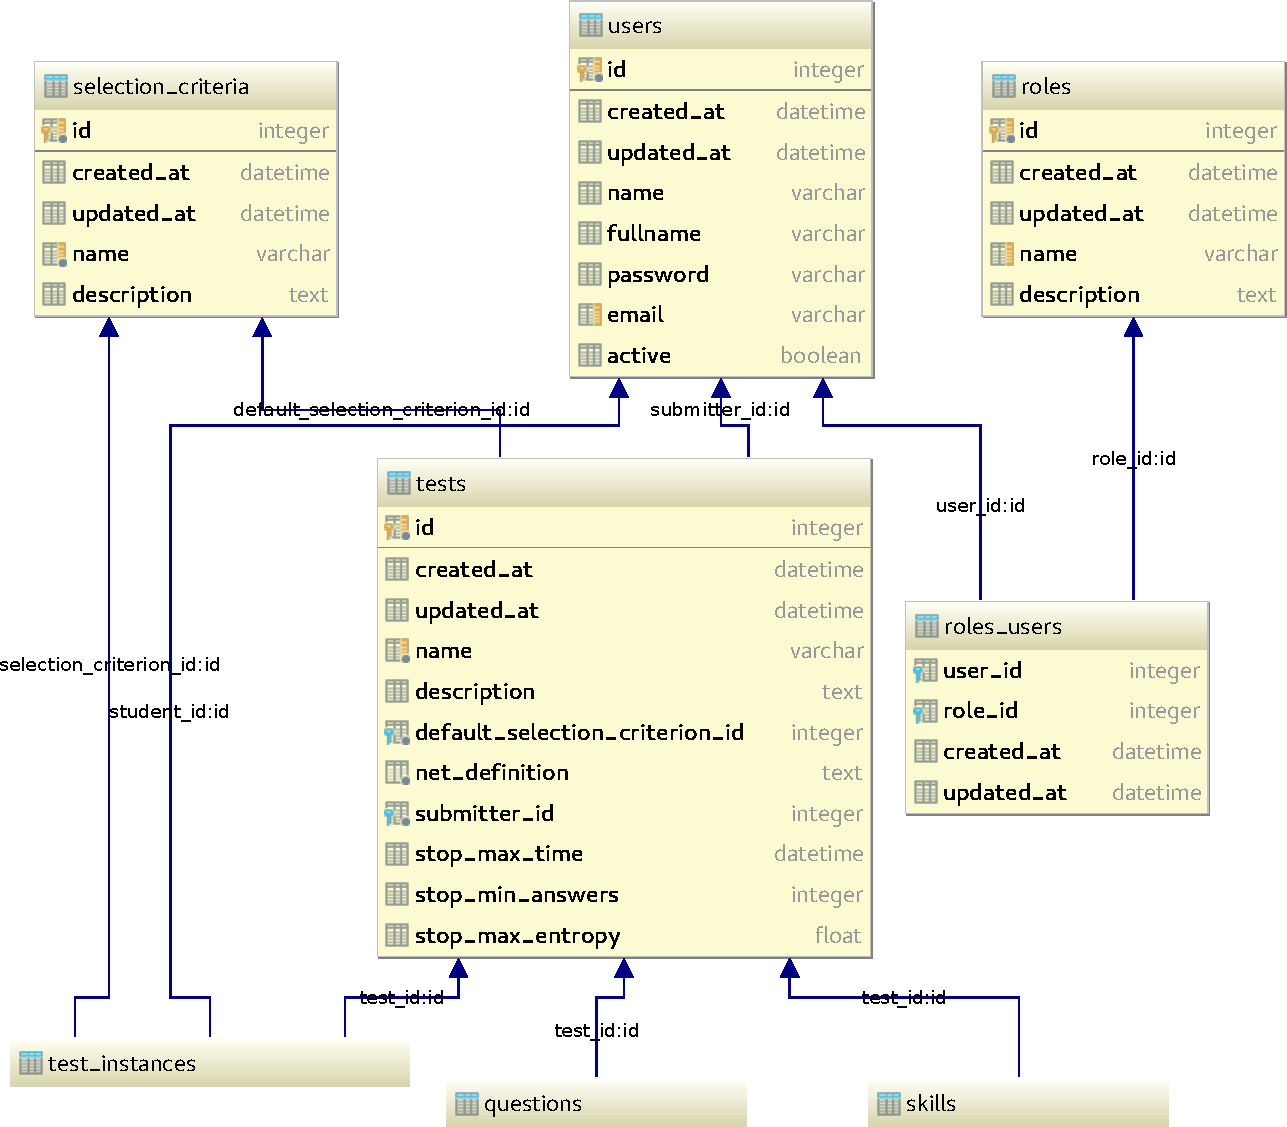
\includegraphics[scale=0.35]{data_model_very_top_only}
\par\end{center}

\end{frame}
%
\begin{frame}{Datový model (2/3)}


\begin{center}
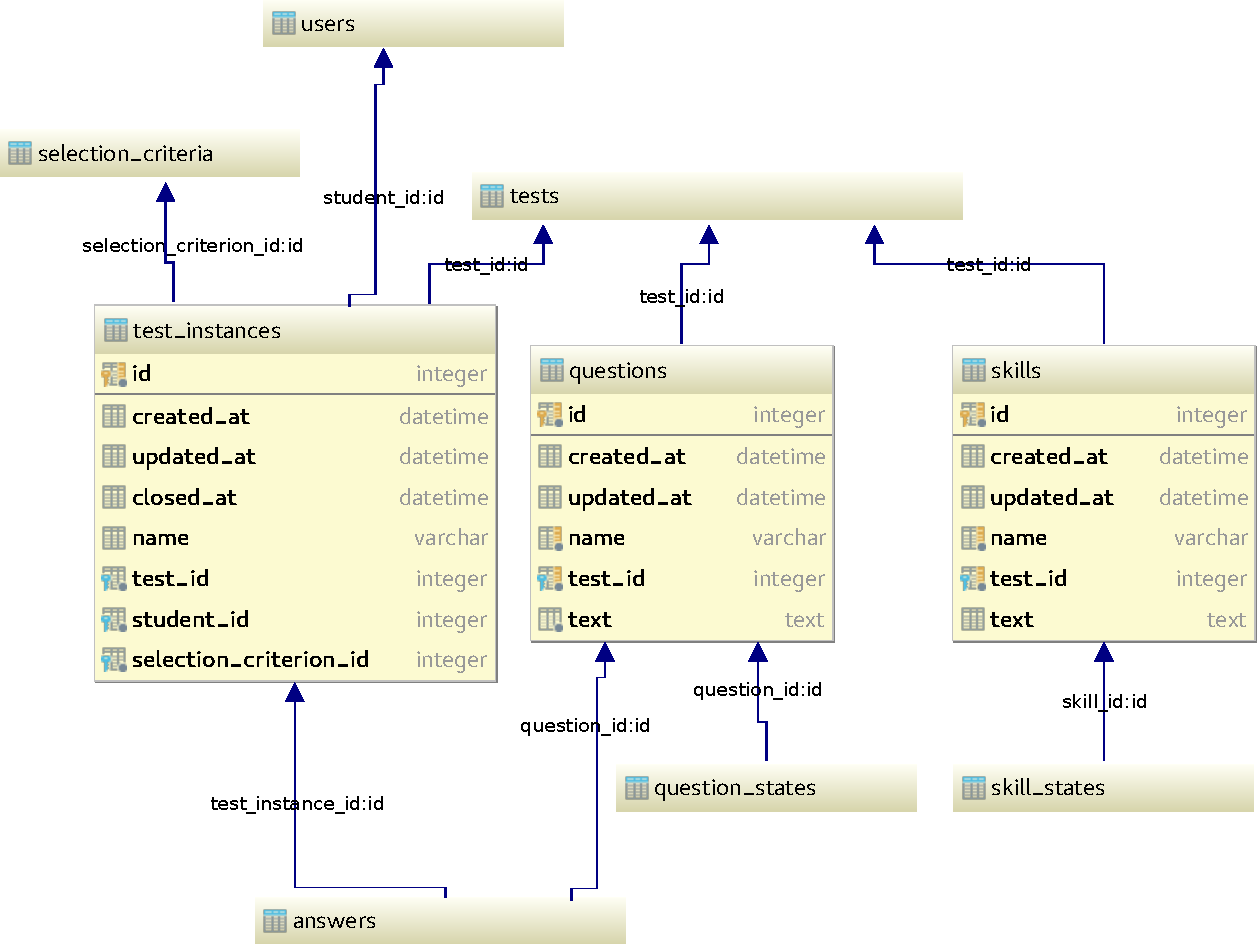
\includegraphics[scale=0.35]{data_model_middle_only}
\par\end{center}

\end{frame}
%
\begin{frame}{Datový model (3/3)}


\begin{center}
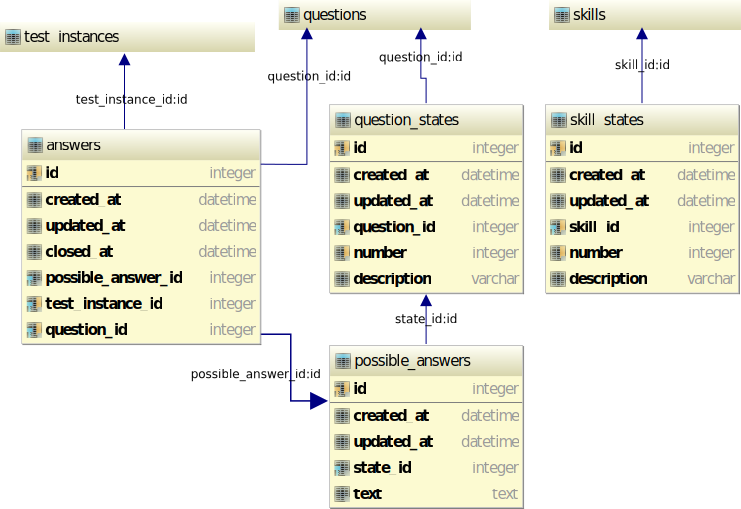
\includegraphics[scale=0.35]{data_model_bottom_only}
\par\end{center}
\end{frame}

\subsection{Rozhraní s R}
\begin{frame}[fragile]{Fragmenty kódu R v Pythonu}
\begin{minted}[fontsize=\footnotesize]{python}
ro.r('''get.marginals <- function(model, node_vector) {
                model <- one.dimensional.marginals(model,
                            node.index(model, node_vector))
                x <- list()
                for(i in 1:length(node_vector)){
                    x[[i]] <- model@marginals[[i]]@a
                }
                x
            }''')
r_get_marginals = ro.r['get.marginals']
\end{minted}
\end{frame}

\begin{frame}[fragile]{Ukázka volání R z Pythonu}
\begin{minted}[fontsize=\footnotesize]{python}
r_pick_question = ro.r['pick.question']


def pick_question(model, all_questions: List[str],
                  candidate_questions: List[str],
                  selection_criterion: int = 1):
    r_all_questions = ro.StrVector(all_questions)
    r_candidate_questions = ro.StrVector(candidate_questions)
    pick_obj = r_pick_question(model, r_all_questions,
                               selection_criterion,
                               r_candidate_questions)
    question_indices = list(pick_obj[2])
    picked_questions = [candidate_questions[index - 1] for index in
                        question_indices]
    return picked_questions
\end{minted}
\end{frame}

\subsection{Webové rozhraní}
\begin{frame}[fragile]{Ukázka pohledové funkce}
\begin{minted}[fontsize=\scriptsize]{python}
@app.route('/test/<int:test_id>')
@login_required
def test_overview(test_id):
    test: Test = get_entity_by_type_and_id(Test, test_id)
    check_test_existence_and_redirect_if_not_exists(test)
    test_instances = list_test_instances_by_test_and_student(test,
                                                             current_user)
    possible_criteria = list_selection_criteria()
    test_instance_options_form = \
        TestInstanceOptionsForm(possible_criteria=[(sc.id, sc.name) for sc
                                                   in possible_criteria],
                                default_criterion=
                                    test.default_selection_criterion.id)
    return render_template("test_overview.html", test=test,
                           test_instances=test_instances,
                           test_instance_options_form=
                               test_instance_options_form,
                           possible_criteria=possible_criteria)
\end{minted}
\end{frame}

\begin{frame}[fragile]{Ukázka z Jinja šablony}
\begin{minted}[fontsize=\footnotesize]{html}

<article>
    <div class="row">
        <div class="six columns">
            <p>Název případu: {{ test_instance.name }}</p>
            <p>Případ zahájen: {{ test_instance.created_at }}</p>
        </div>
        <div class="six columns">
            <a class="button"
              href="{{ url_for('test_instance_overview',
                               test_id=test.id,
                               test_instance_id=test_instance.id) }}">
                Otevřít přehled případu</a>
        </div>
    </div>
</article>

\end{minted}
\end{frame}

\subsection{Pracovní postup studenta}
\begin{frame}{Postup testování}
\begin{enumerate}
\item Student je odkázán na web nebo konkrétní test,
\item student si vybere ručně, nebo je mu vybrána systémem otázka, \label{step:rep}
\item student zodpoví otázku,
\item pokud je dosaženo ukončovacího kritéria (čas, počet otázek, entropie), test končí, jinak následuje krok \ref{step:rep}.
\end{enumerate}
Výsledky testu jsou vidět průběžně i po jeho ukončení.
\end{frame}

\subsection{Analýza časové náročnosti}
\begin{frame}{Problémy s časovou náročností}
Problémy:
\begin{itemize}
  \item Jen když je potřeba použít \texttt{catest},
  \item \textit{R} hodně kopíruje data (předávání argumentů funkcím),
  \item \texttt{catest} není příliš optimalizována.
\end{itemize}
Možná řešení:
\begin{itemize}
  \item Asynchronní předpočítávání možných scénářů vývoje testu,
  \item rychlejší implementace \texttt{catest} (asi v něčem jiném než \textit{R}),
  \item provedení optimalizace \texttt{catest}.
\end{itemize}
\end{frame}

\subsection{Budoucí vývoj}
\begin{frame}{Možnosti budoucího vývoje}
Chybí:
\begin{itemize}
  \item Nástroje pro analýzu výsledků (dat je ovšem dost),
  \item webové rozhraní pro zadávání testů a
  \item webové rozhraní pro administraci.
\end{itemize}
Další postup:
\begin{itemize}
  \item Navrhnout strojově čitelný formát pro zadávání testu,
  \item navrhnout analytické nástroje,
  \item implementovat příslušná rozhraní a nástroje.
\end{itemize}
\end{frame}

\section{Závěr}
\subsection{Vlastní zhodnocení}
\begin{frame}{Vlastní zhodnocení výzkumného úkolu}
\begin{itemize}
  \item Zajímavé koncepty (mám zájem o zefektivnění učení),
  \item mnoho nabytých zkušeností s vývojem aplikací,
  \item \textit{Flask} a přidružené knihovny výbornými nástroji,
  \item do budoucna možný velký vývoj:
  \begin{itemize}
    \item jako zpětná vazba pro studenty a vyučující,
    \item případně jako základ automatického systému pro výuku,
    \item nebo i jako obecného psychometrického systému.
  \end{itemize}
\end{itemize}
\end{frame}

\begin{frame}[plain]
\begin{center}
{\huge \textbf{Děkuji za pozornost a věnovaný čas.}}
\end{center}
% \tableofcontents
\end{frame}

\end{document}
